\documentclass[UTF8]{ctexart}
\usepackage{ctex}
\usepackage{geometry}
\geometry{left=3.18cm,right=3.18cm,top=2.54cm,bottom=2.54cm}
\usepackage{graphicx}
\usepackage{framed}
\usepackage{fancyhdr}
\usepackage{setspace}
\pagestyle{fancy}%清除原页眉页脚样式
\fancyhf{}
\fancyhead[C]{华中科技大学电信学院}
\fancyfoot[C]{\thepage}
% \pagestyle{plain}
\begin{document}
\begin{center}
    \quad \\
    \quad \\
    % \kaishu \fontsize{35}{5} \textbf{华 中 科 技 大 学}
    % \vskip 3cm
    \fangsong \fontsize{49}{5}《通信电子线路》实验报告
    \vskip 3cm
    \heiti \zihao{1}\textbf{高频谐振功率}
    \fangsong \zihao{1} 放大器仿真
\end{center}

\makeatletter
\newcommand\dlmu[2][4cm]{\hskip1pt\underline{\hb@xt@ #1{\hss#2\hss}}\hskip3pt}
\makeatother

\vskip 3cm
\begin{center}
    \zihao{3}
    \begin{tabular}{rl}
         & \makebox[4em][s]{学生姓名}	\hspace{0.2cm}	\dlmu[9cm]{赵展}
         \\
         & \makebox[4em][s]{学号}	\hspace{0.2cm}	\dlmu[9cm]{U202117282}
         \\
         & \makebox[4em][s]{专业班级}	\hspace{0.2cm}		\dlmu[9cm]{种子2101班}
         \\
         & \makebox[4em][s]{实验平台}	\hspace{0.2cm}		\dlmu[9cm]{Multisim 14.3 on Windows}
         \\
    \end{tabular}
    \vskip 3cm
    2023年10月26日
\end{center}

\newpage
\tableofcontents
\newpage
\section{实验目的}
\begin{itemize}
    \item 进一步熟悉NIMultisim电路仿真软件的使用
    \item 掌握高频谐振功率放大器的电路结构特点及工作原理
    \item 熟悉高频谐振功率放大器的调谐方法
    \item 熟悉高频谐振功率放大器的三种工作状态及调整方法
\end{itemize}
\section{实验内容}
\begin{itemize}
    \item 使用NIMultisim 绘制高频谐振功率放大器的仿真电路
    \item 进行时域仿真,观察时域波形,体现基极回路反偏状态
    \item 进行频域仿真,分析电路频域响应
    \item 测试高频谐振功放中欠压和过压工作状态之间的不同
    \item 要求输入信号频率至少为10MHz
\end{itemize}
\section{实验原理}
高频谐振功率放大电器原理电路如图\ref{img:1}所示,电路由晶体管、LC谐振回路与直流供电电路
组成,晶体管在将供电电源的直流能量转变为交流能量的过程中起开关控制作用,谐振回路
LC 是晶体管的负载,直流供电电路为各级提供适当工作状态和电源,其中$V_{BB}$是基极偏置,
$V_{CC}$是集电极电源,晶体管工作状态为丙类。
\begin{figure}[htbp]
    \centering
    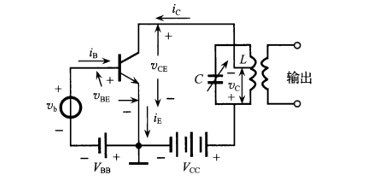
\includegraphics{1.png}
    \caption{高频谐振功率放大器原理图}
    \label{img:1}
\end{figure}
\section{实验步骤}
\begin{enumerate}
    \item 按照实验原理图,搭建仿真实验电路
    \item 验证静态工作点
    \item 观察时域波形:启动仿真后,开启示波器,观察输入输出波形;使用瞬态分析,添加输入输出的电压值,晶体管的集电极电流(经过倍数处理)作为观察量,启动仿真
    \item 观察频域特性:分别对输入输出信号使用傅里叶分析,观察其频谱图;使用交流分析,添加AV 为其观察量,得到幅频响应曲线与相频响应曲线,并标出其通频带
    \item 改变$V_{BB}$ 或$V_1$的值,分别让功放工作在欠压/临界/过压状态下,重复上述仿真
\end{enumerate}
\section{实验结果与分析}
\subsection{时域特性}
\subsubsection{直流工作点分析}
根据上述原理图可以在Multisim中搭建如图\ref{img:2}的仿真电路。
启动直流静态工作点进行仿真得到如图\ref{img:3}所示的结果:
其中可以看到晶体管的$I_B,I_C,I_E$,基极和集电极电压,此时基极电压$V_3$的值为-1V表明基极回路处于反偏状态。
/\begin{figure}[htbp]
    \centering
    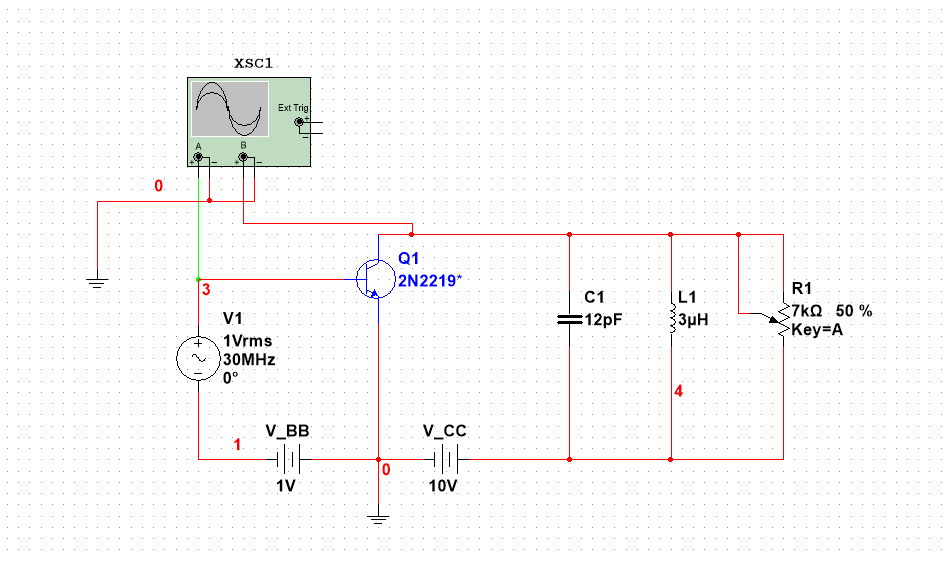
\includegraphics[width=0.8\textwidth]{2.png}
    \caption{高频谐振功率放大器仿真电路}
    \label{img:2}
\end{figure}
\begin{figure}[htbp]
    \centering
    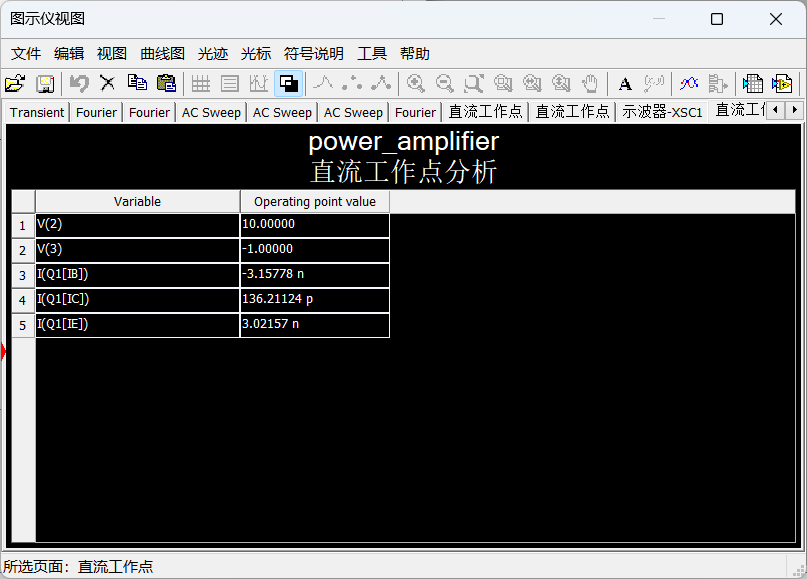
\includegraphics[width=0.8\textwidth]{3.png}
    \caption{直流工作点}
    \label{img:3}
\end{figure}
\subsubsection{输入输出信号波形}
运行电路,查看示波器的结果如图\ref{img:4}所示,
\begin{figure}[htbp]
    \centering
    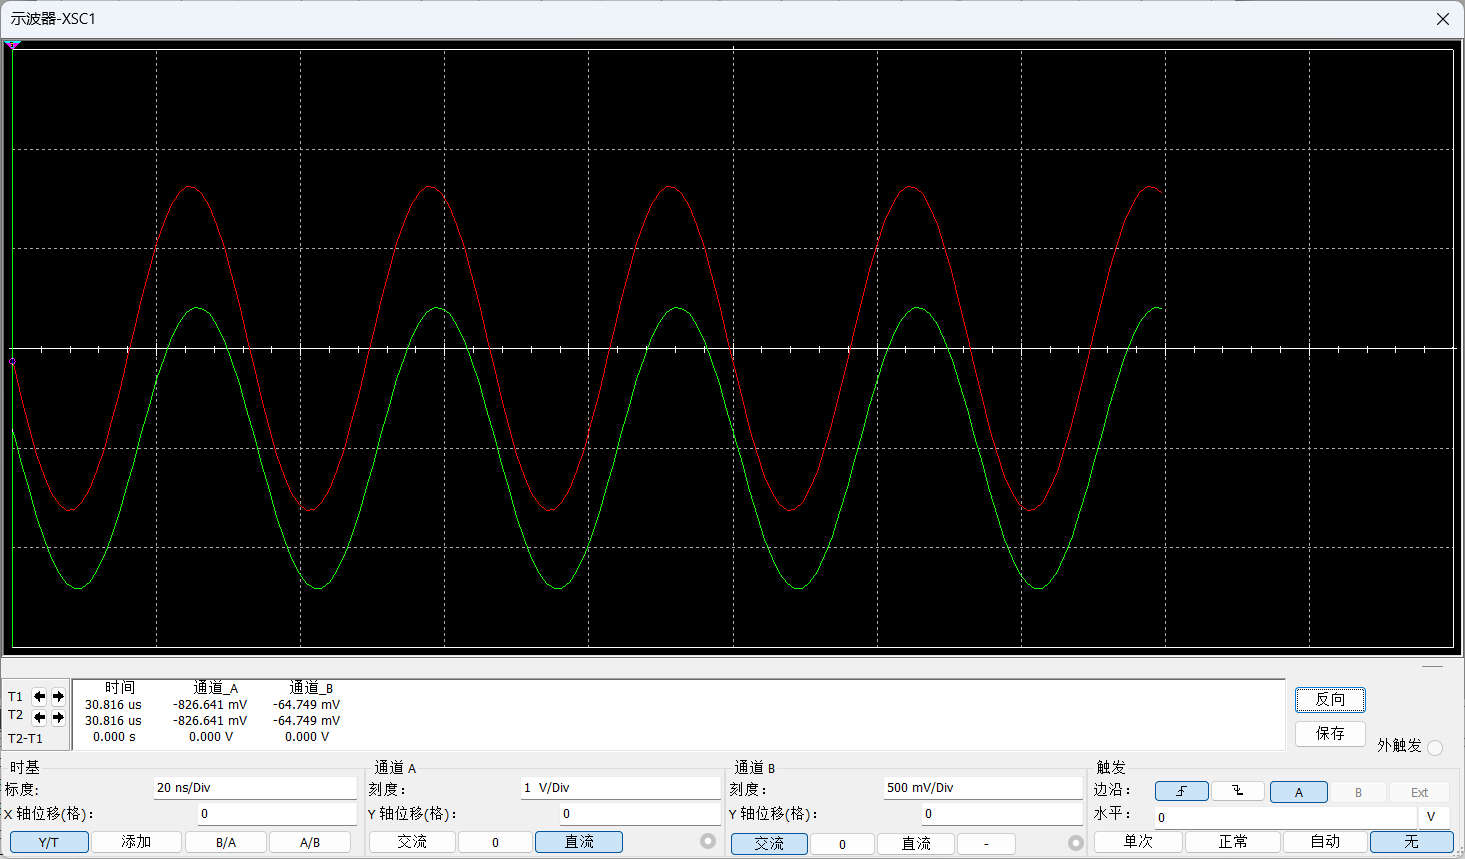
\includegraphics[width=0.8\textwidth]{4.png}
    \caption{示波器:输入输出信号波形}
    \label{img:4}
\end{figure}
其中绿色波形为通道A,连接的是输入信号,采用的是直流输入,可以看到有一个负的直流偏置,该偏置来自于基极的反偏电压$V_{BB}$,体现了基极回路的反偏状态;
红色波形为通道B,连接的输出型号,采用交流输入,为完整的正弦波,说明其工作在欠压区
\subsection{频域特性}
\subsubsection{傅里叶分析-频谱}
选择傅里叶分析,添加输入信号和输出信号为观察量,启动仿真,得到输入输出信号的频谱如图\ref{img:5}和\ref{img:6}所示。
\begin{figure}[htbp]
    \centering
    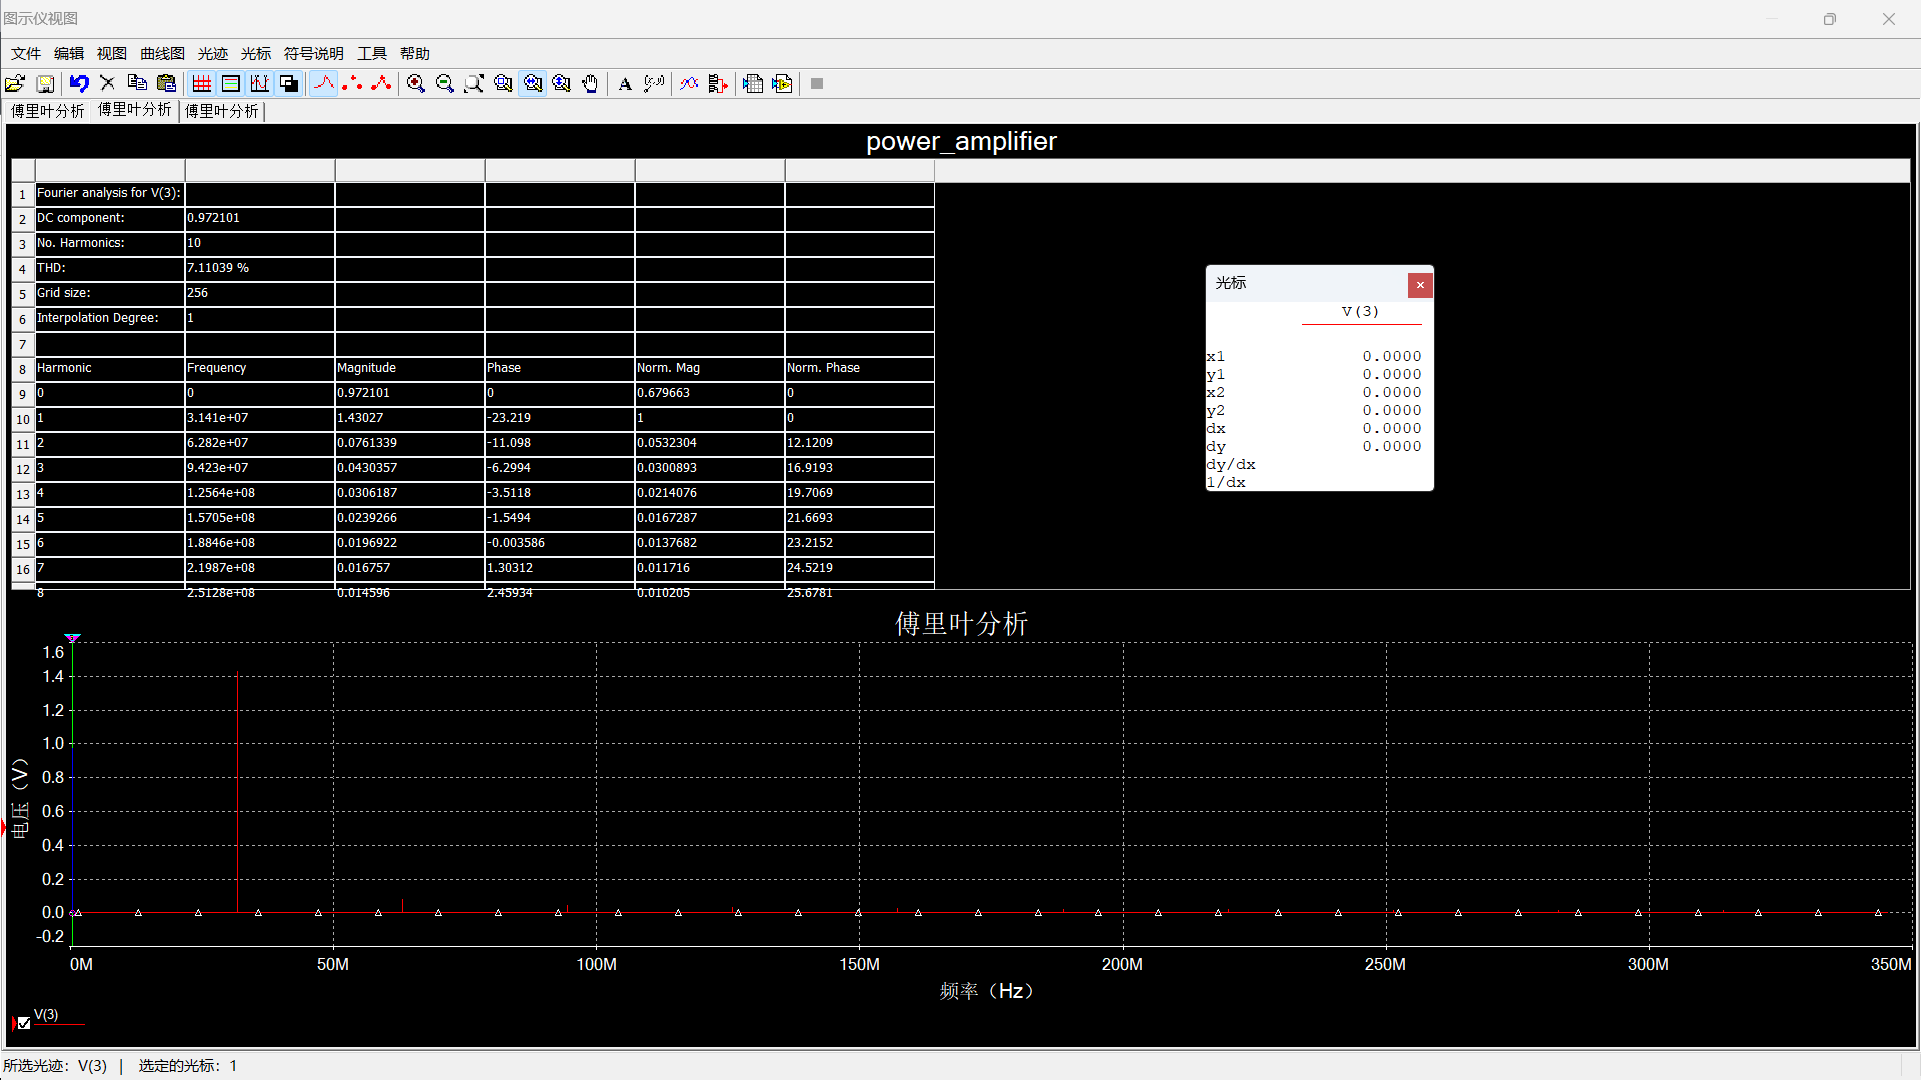
\includegraphics[width=0.8\textwidth]{5.png}
    \caption{傅里叶分析:输入信号}
    \label{img:5}
\end{figure}
\begin{figure}[htbp]
    \centering
    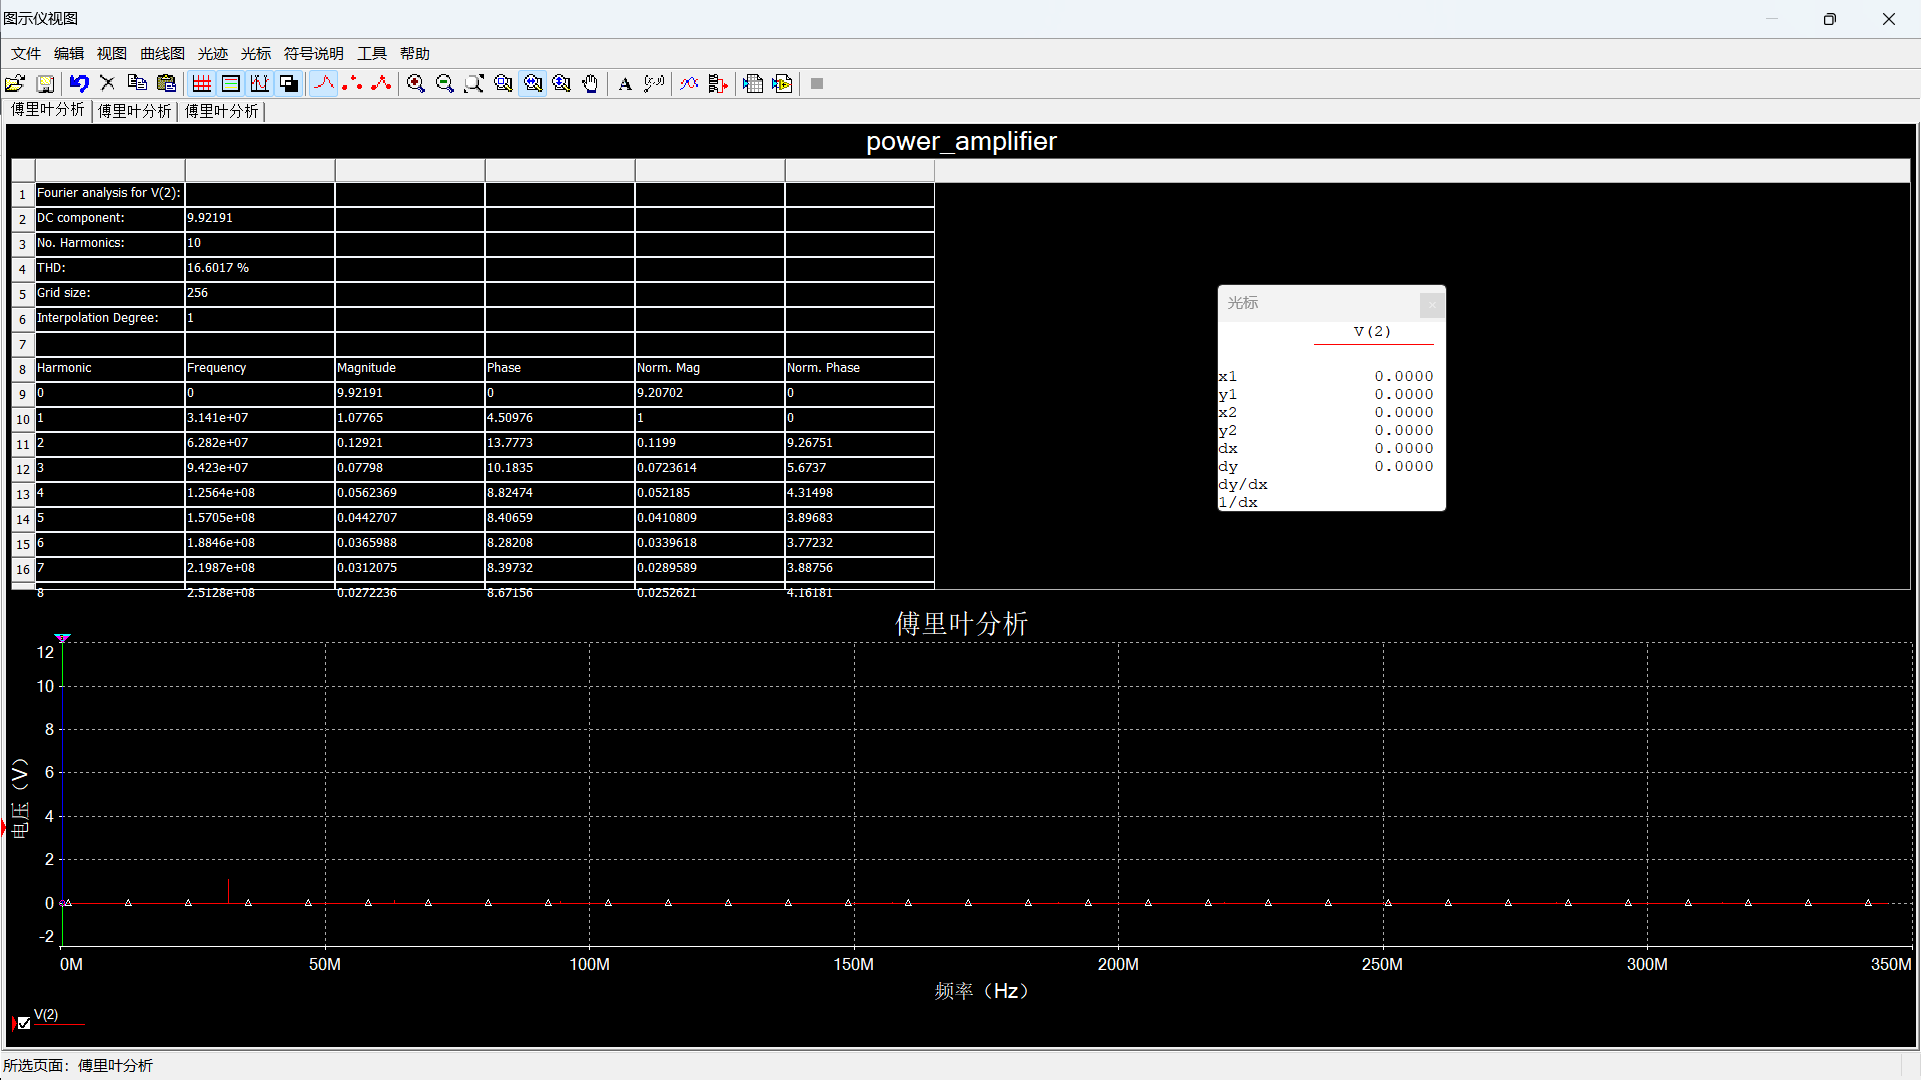
\includegraphics[width=0.8\textwidth]{6}
    \caption{傅里叶分析:输出信号}
    \label{img:6}
\end{figure}
\subsubsection{交流分析-幅相响应}
继续对该电路进行交流分析,得到幅频响应曲线与相频响应曲线如图\ref{img:7}:
得到的峰值为1.9541,放大幅频响应曲线,标出峰值的0.707倍(1.9541*0.707=1.382)处,
如图\ref{img:8}所示,可知其通频带:
$$
B=24.7488MHz-21.8203MHz=2.9285MHz
$$
\begin{figure}[htbp]
    \centering
    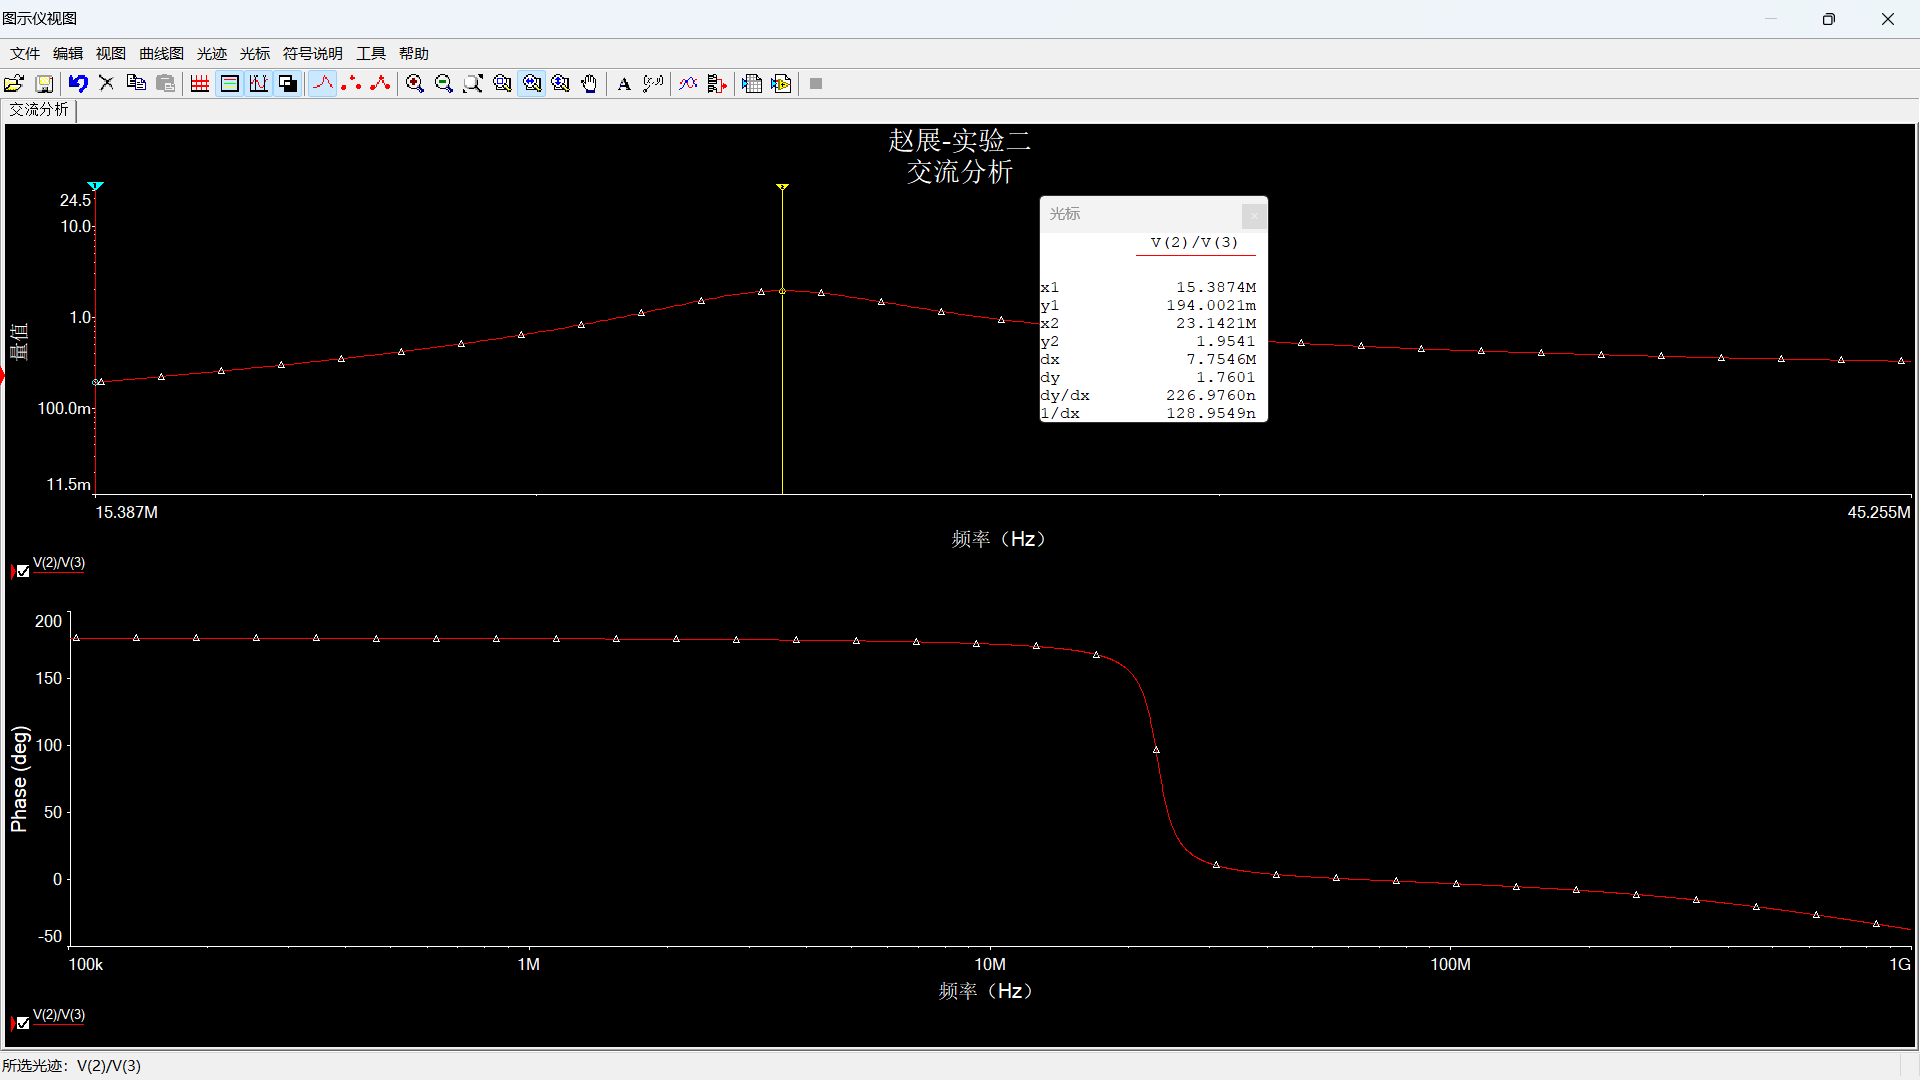
\includegraphics[width=0.8\textwidth]{7.png}
    \caption{交流分析:幅频响应曲线与相频响应曲线}
    \label{img:7}
\end{figure}
\begin{figure}[htbp]
    \centering
    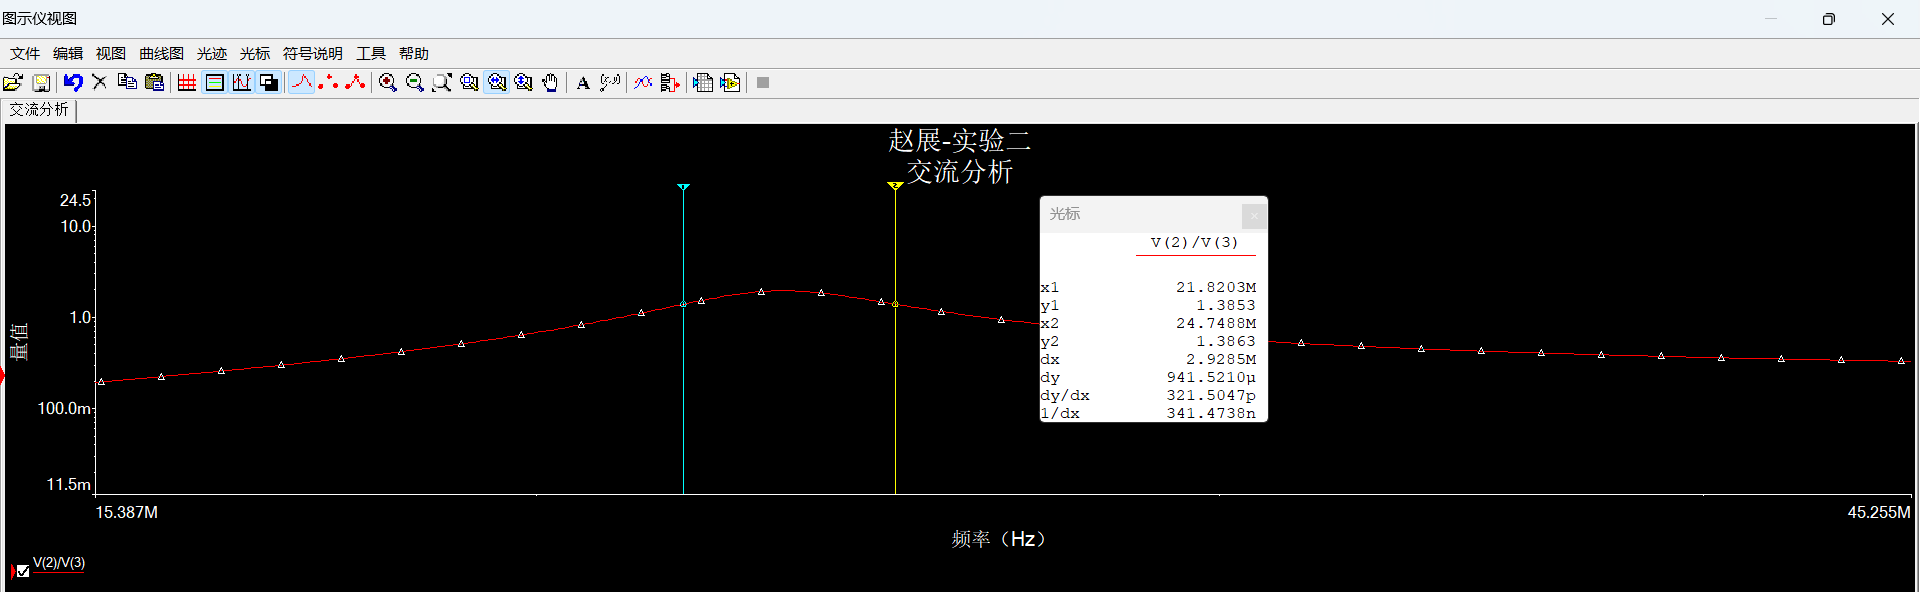
\includegraphics[width=0.8\textwidth]{8.png}
    \caption{交流分析:通频带}
    \label{img:8}
\end{figure}
\subsection{欠压和过压状态}
\subsubsection{过压}
修改$V_1$的有效值为1.2V,重新启动瞬态分析仿真,得到输出集电极电流$i_c$的时域波形如图\ref{img:9}所示,图中标出了导通角的范围,为:
$$
1.1626-1.1402=0.0224\mu s
$$
启动傅里叶分析仿真,添加$i_c$、输入信号、输出信号为观察参数,得到$i_c$、输入信号、输出信号的频谱如图\ref{img:10},\ref{img:11},\ref{img:12}所示,
可以看到,$i_c$频谱出现其他谐波分量,$i_c$出现失真
\begin{figure}[htbp]
    \centering
    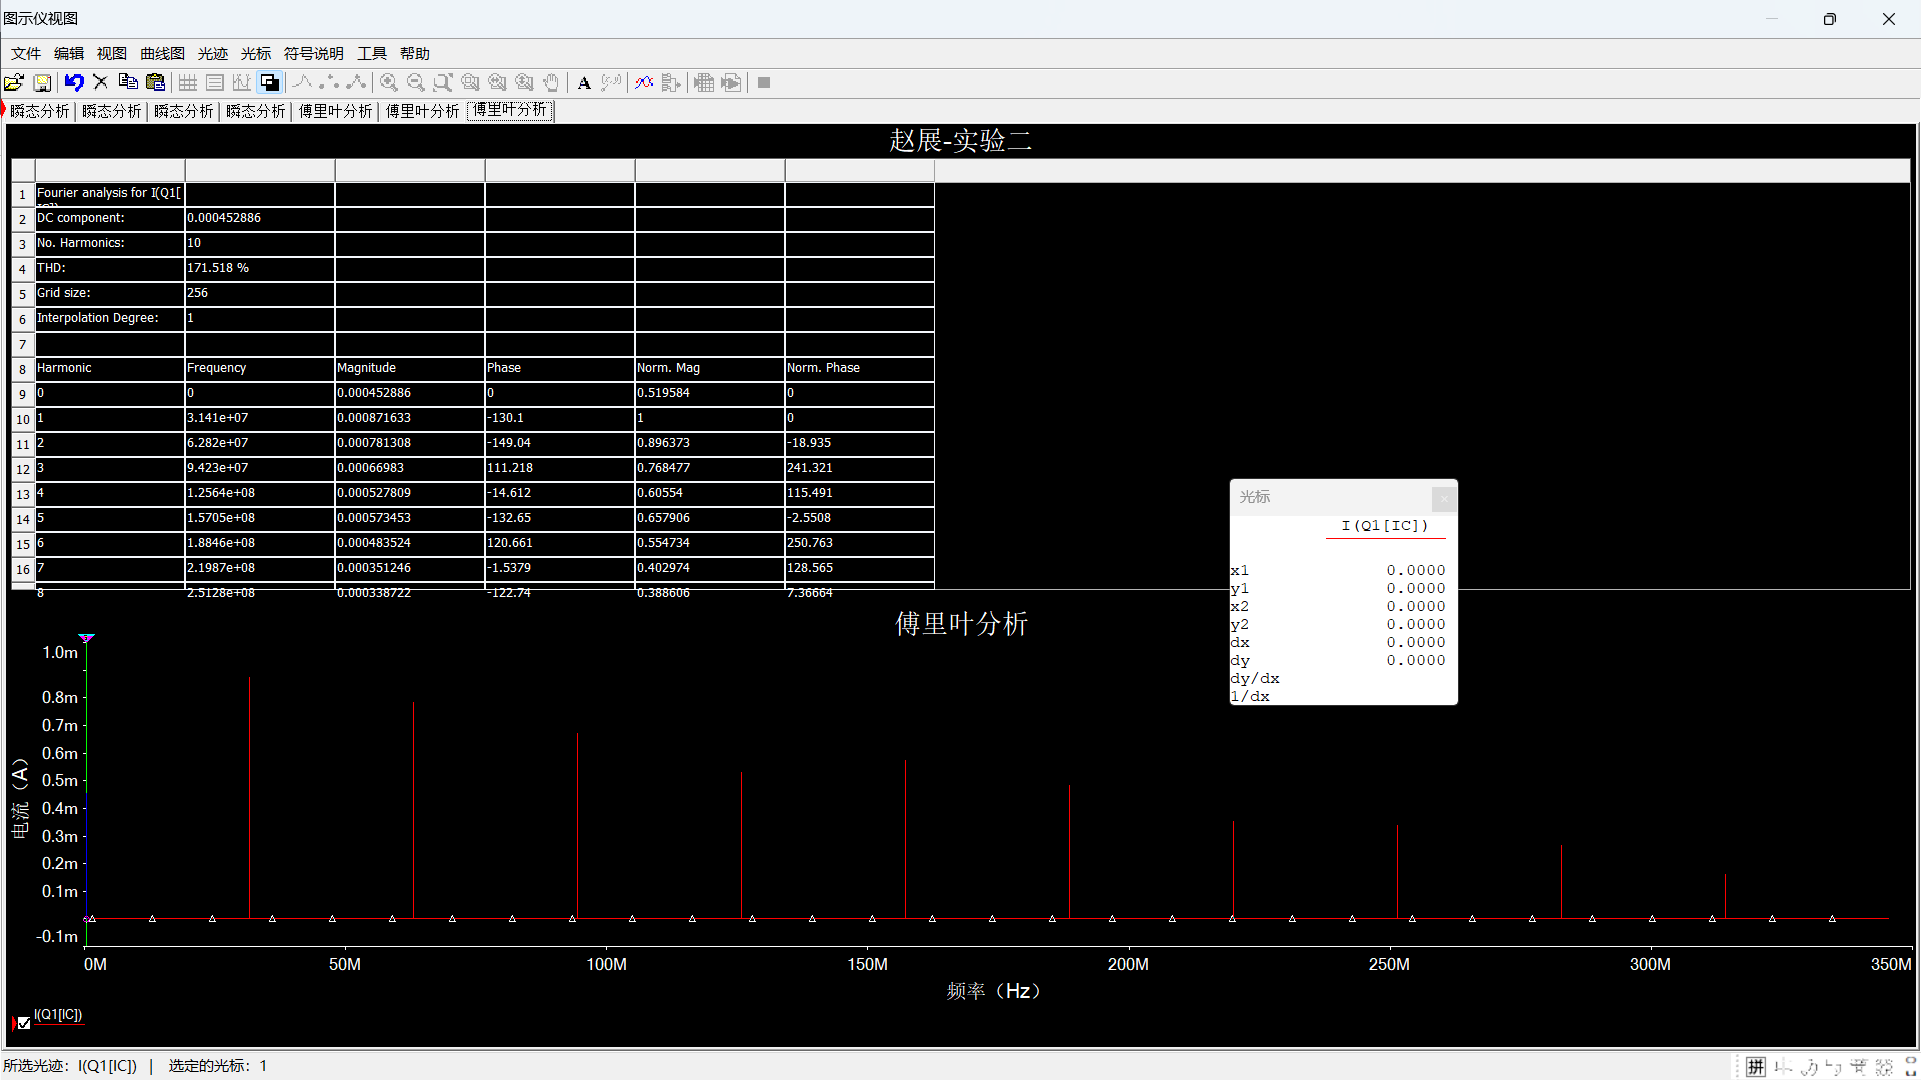
\includegraphics[width=0.6\textwidth]{10.png}
    \caption{傅里叶分析:过压状态$i_c$频谱}
    \label{img:10}
\end{figure}
\begin{figure}[htbp]
    \centering
    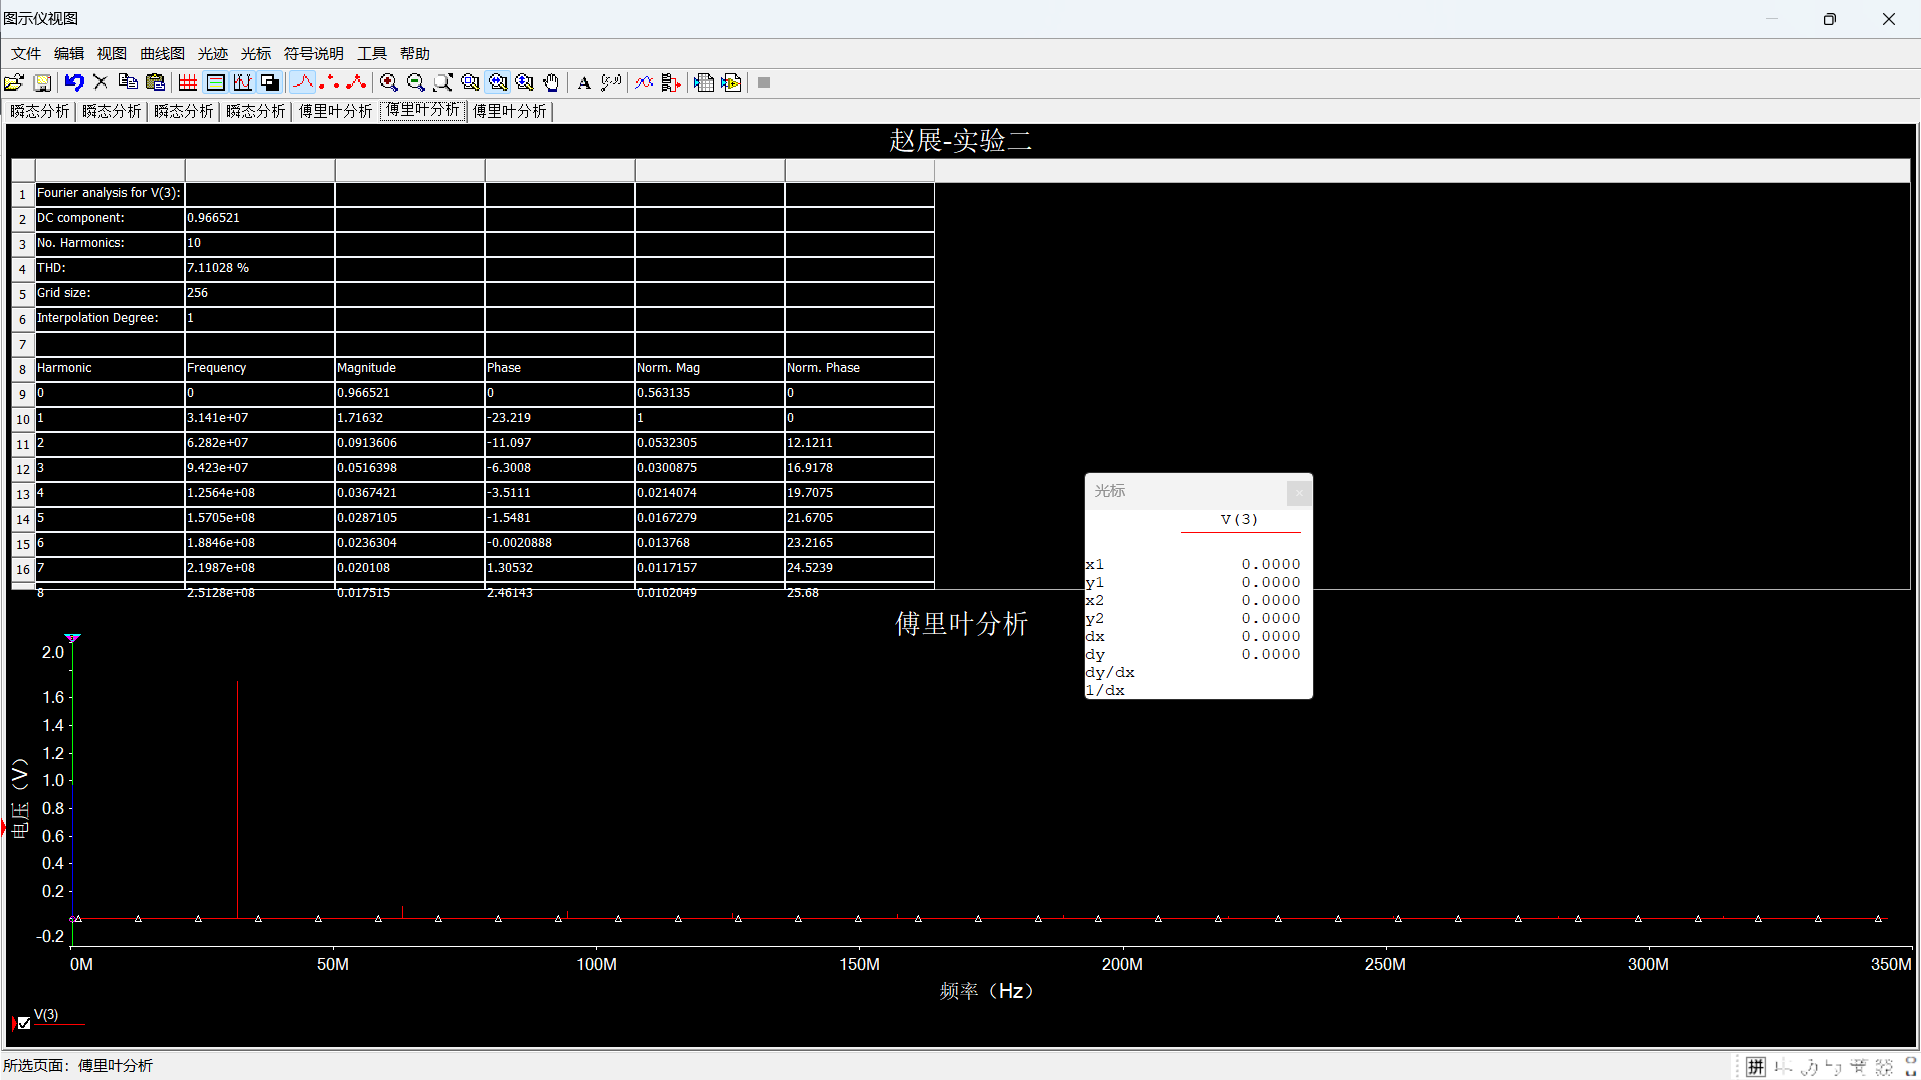
\includegraphics[width=0.6\textwidth]{11.png}
    \caption{傅里叶分析:过压状态输入信号}
    \label{img:11}
\end{figure}
\begin{figure}[htbp]
    \centering
    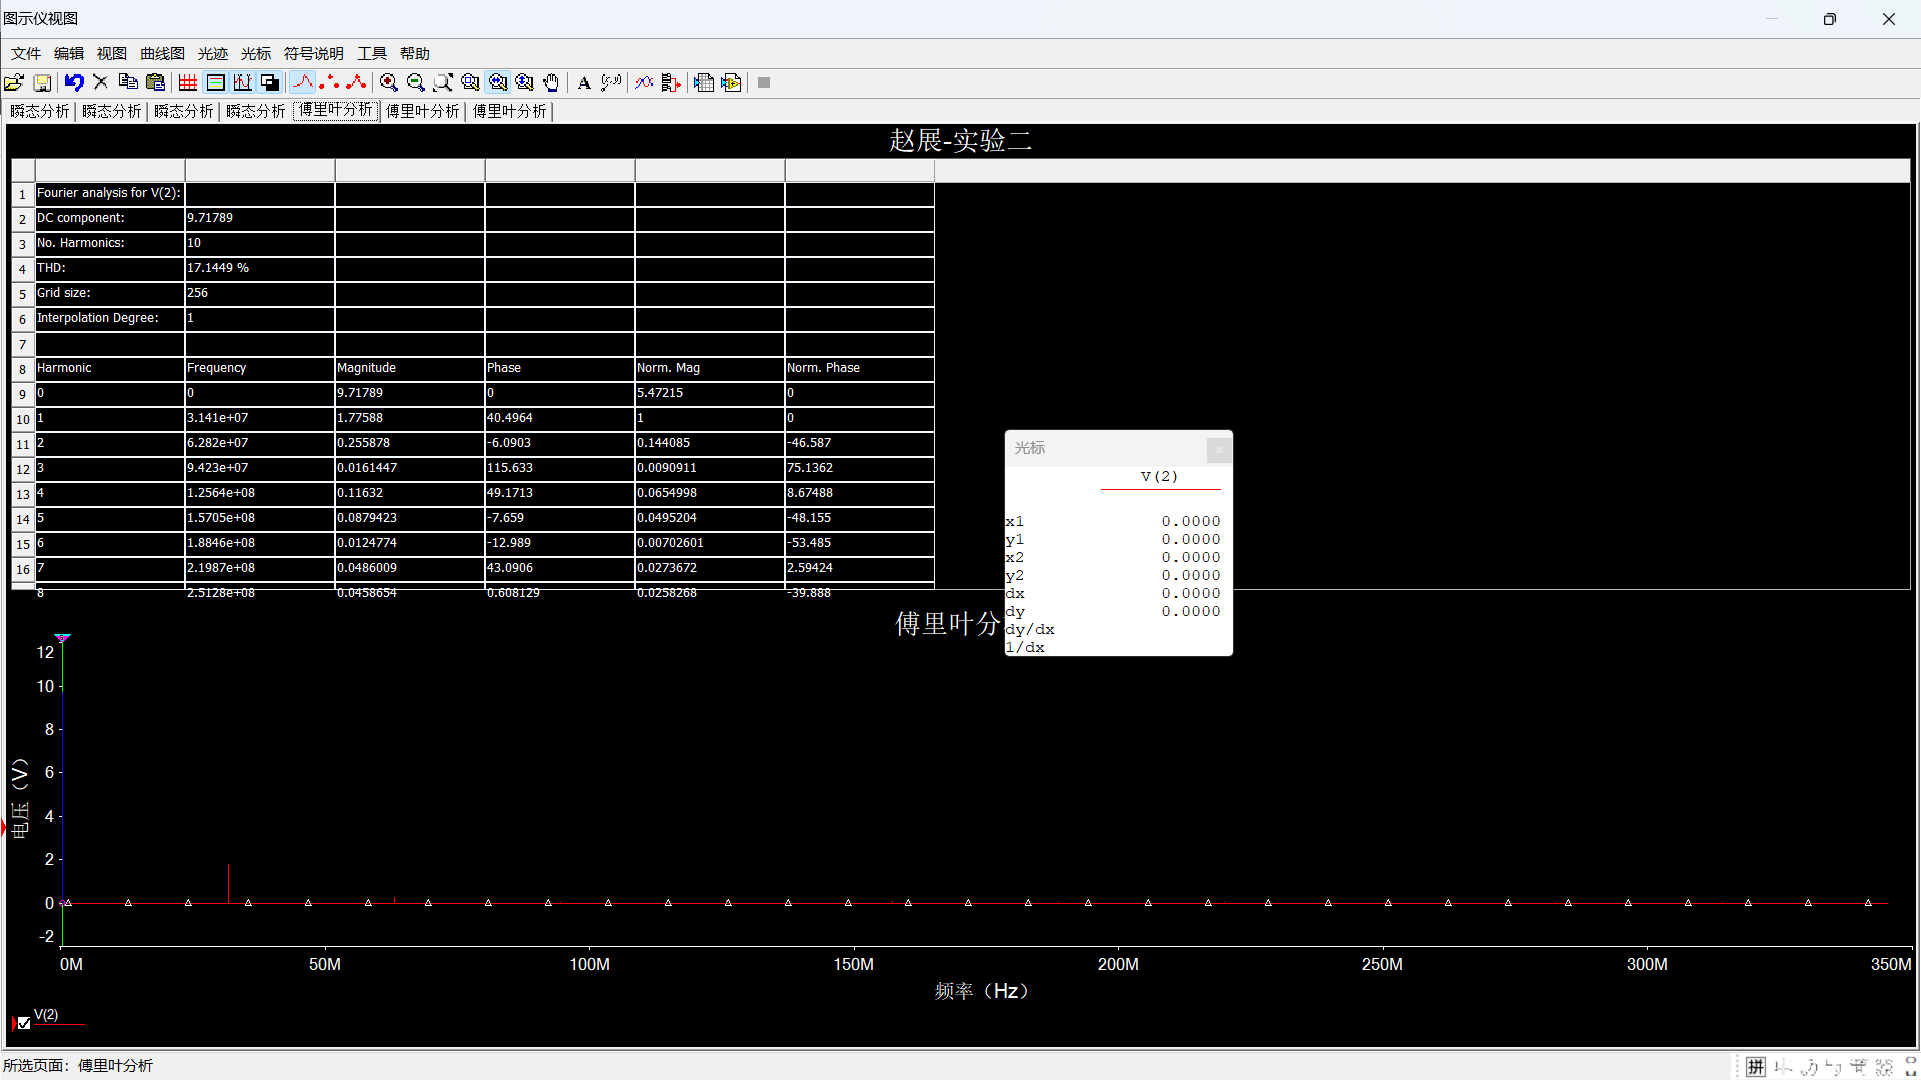
\includegraphics[width=0.6\textwidth]{12.png}
    \caption{傅里叶分析:过压状态输出信号}
    \label{img:12}
\end{figure}
\begin{figure}[htbp]
    \centering
    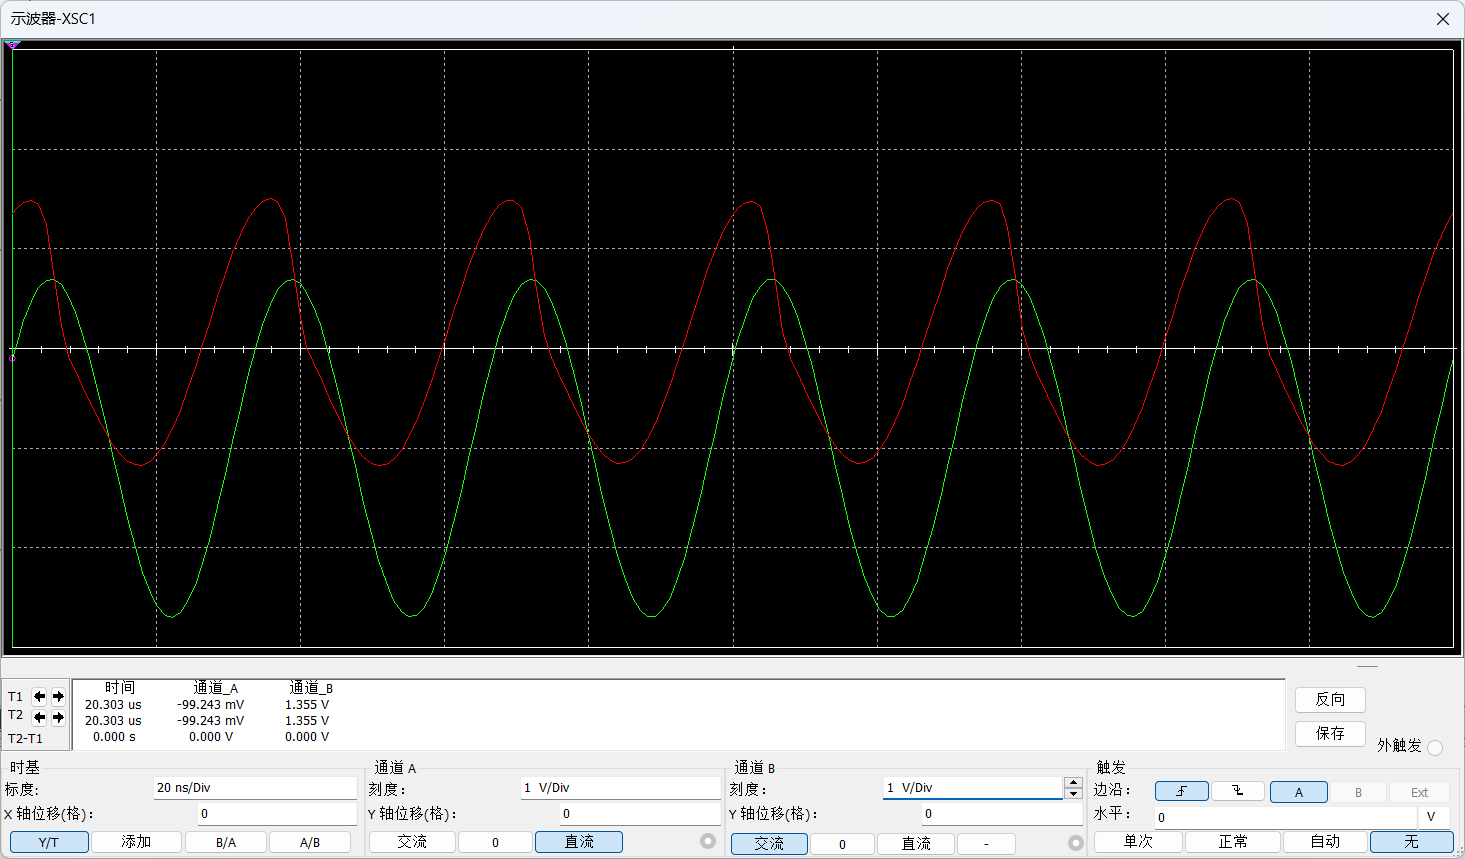
\includegraphics[width=0.8\textwidth]{13.png}
    \caption{示波器:过压状态输入输出信号}
    \label{img:13}
\end{figure}
此时通过示波器查看输入输出信号的时域波形如图\ref{img:13}所示,可以看出输出信号不是完整的正弦波,出现了失真。
\subsubsection{欠压}
修改$V_{CC}$的值为1V,重新启动瞬态分析仿真,得到得到输出集电极电流$i_C$的时域波形如图\ref{img:14}所示,
图中标出了其导通角的范围为:
$$
1.1266-1.1100=0.0166\mu s
$$
\begin{figure}[htbp]
    \centering
    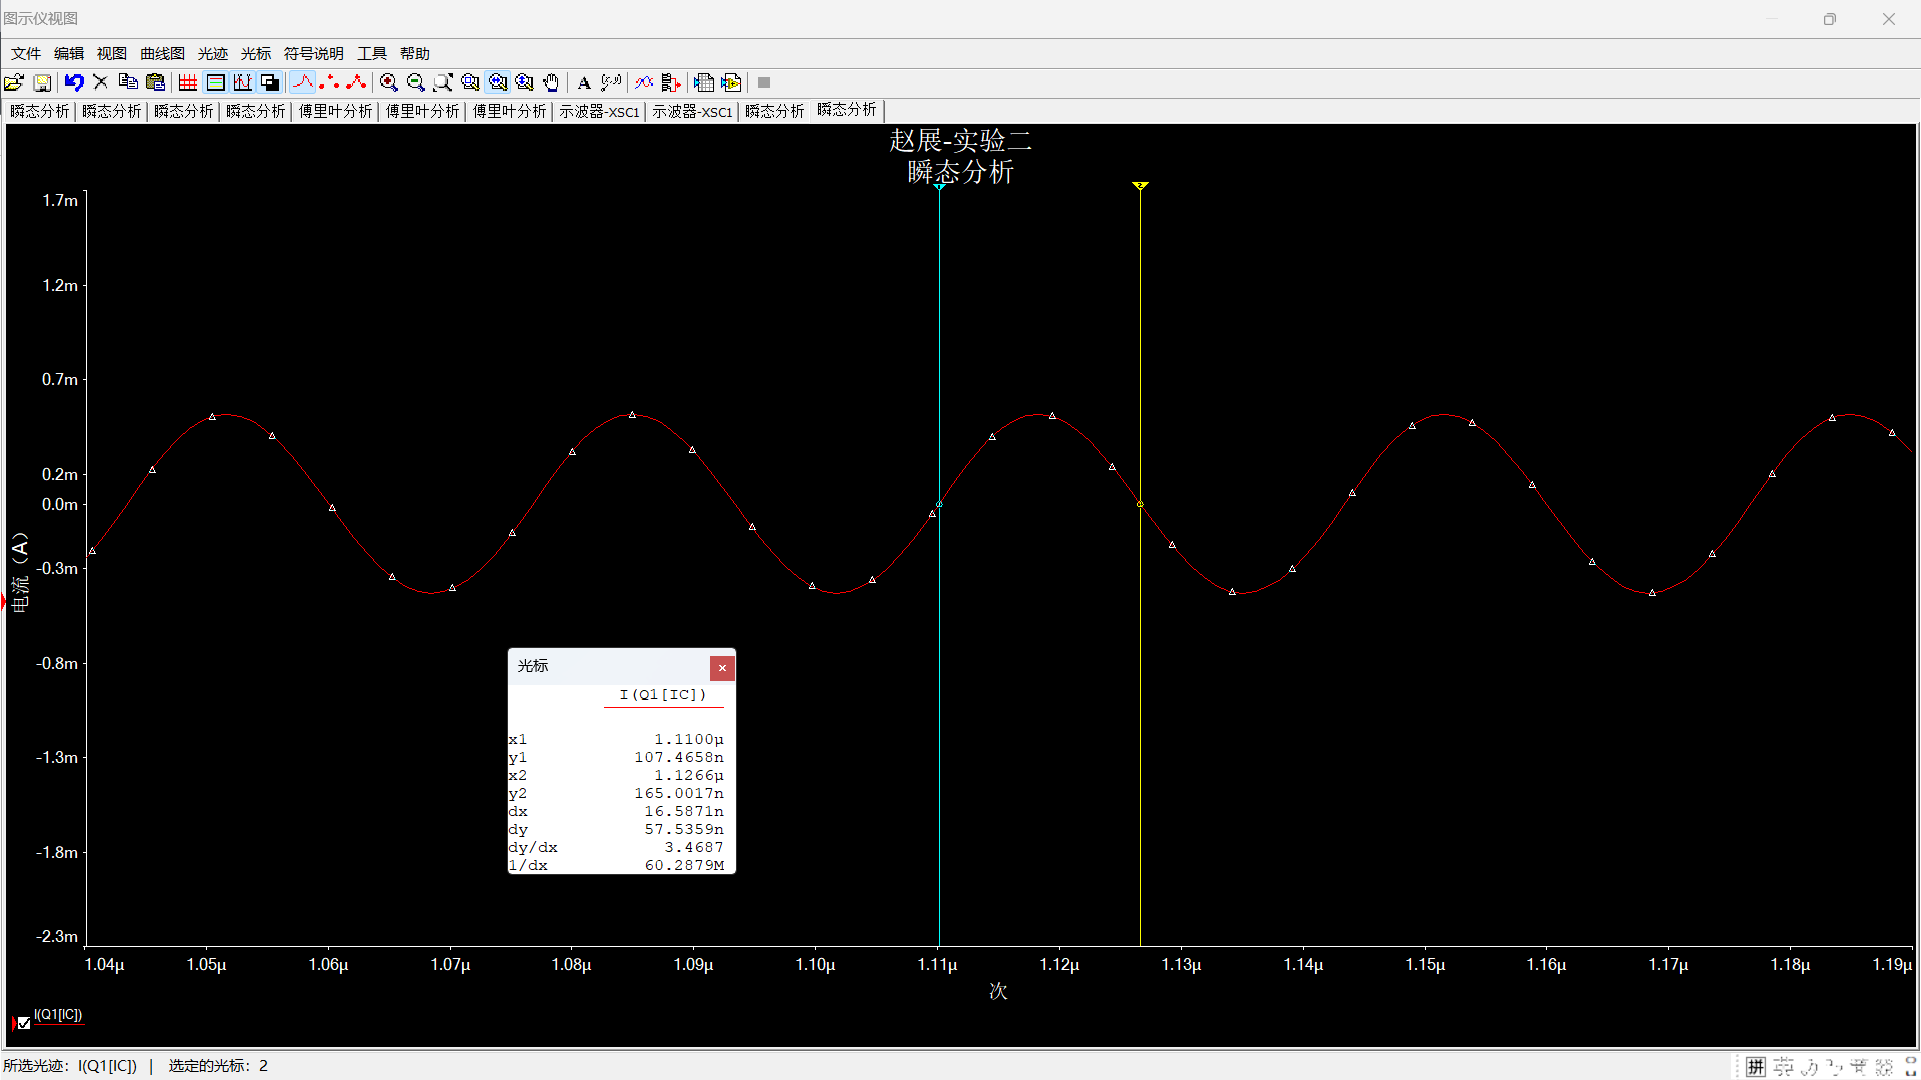
\includegraphics[width=0.8\textwidth]{14.png}
    \caption{瞬态分析:欠压状态$i_c$}
    \label{img:14}
\end{figure}
\begin{figure}[htbp]
    \centering
    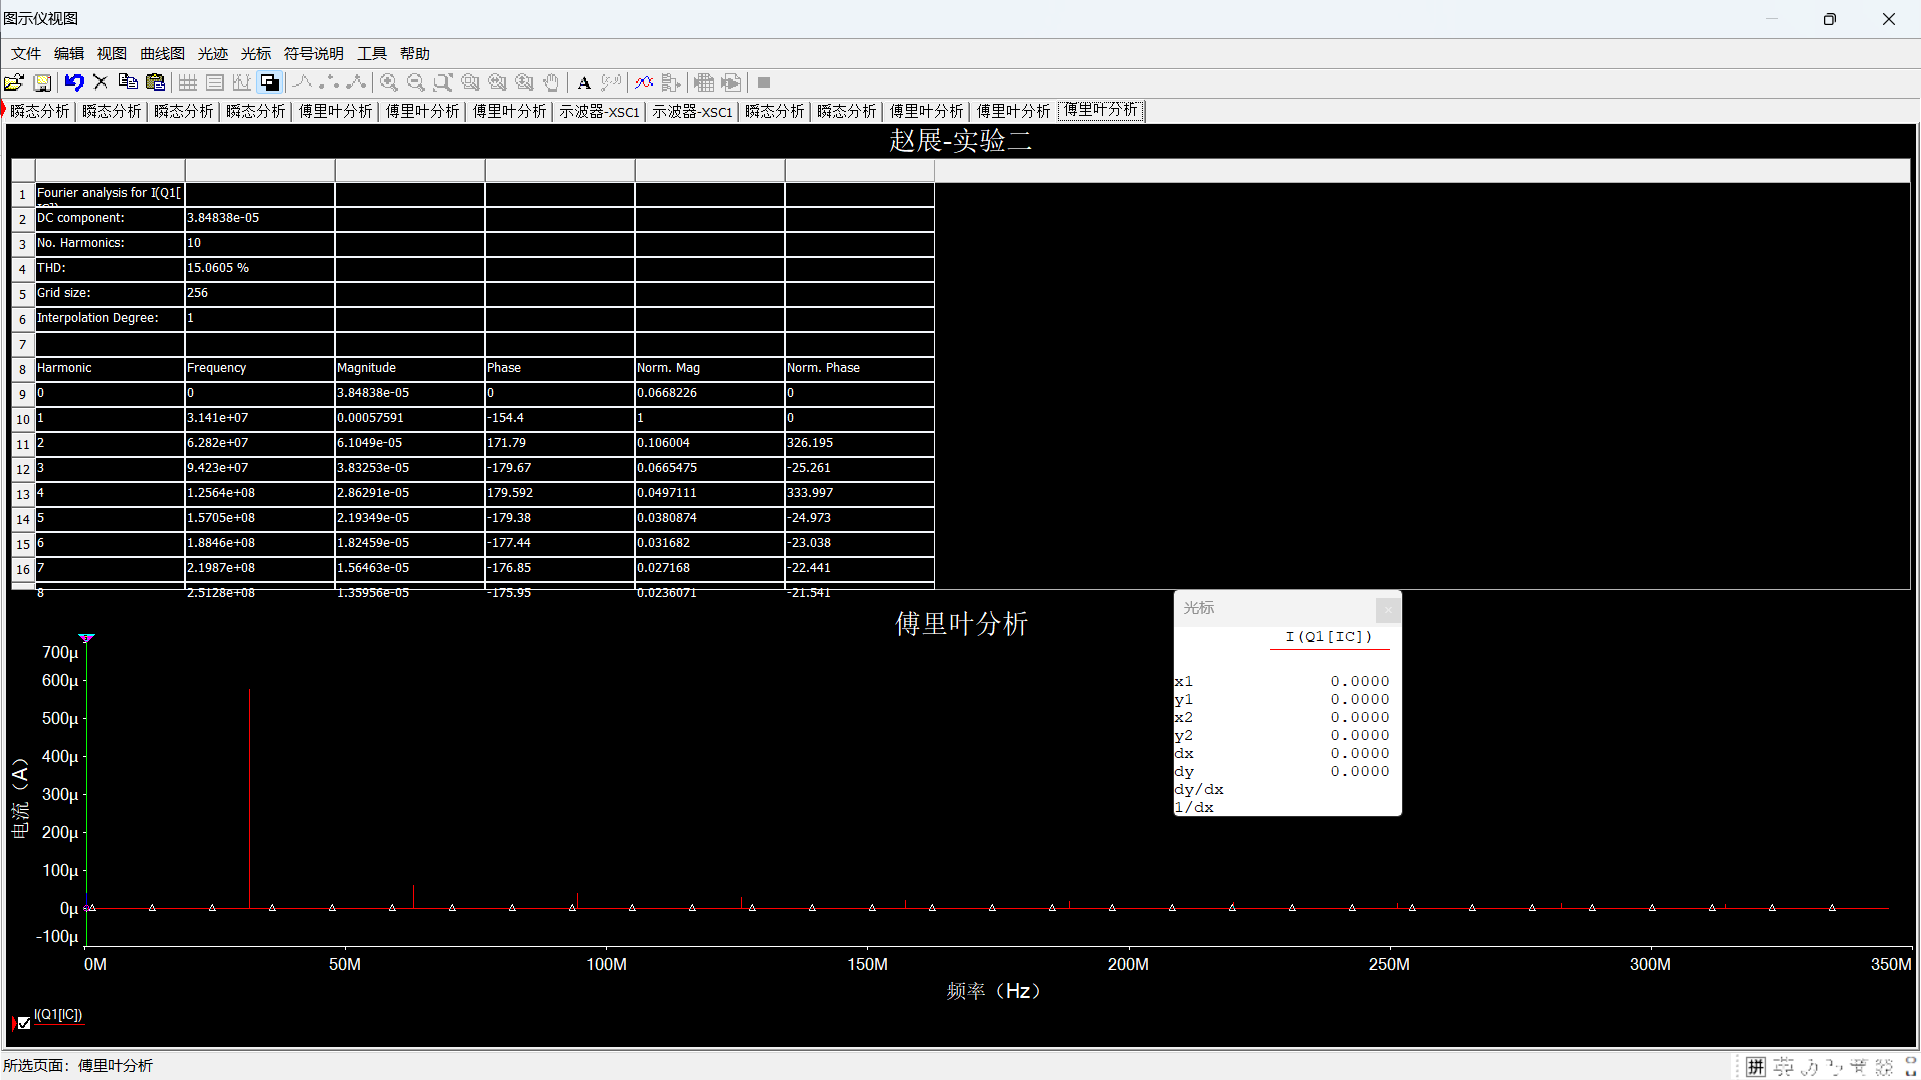
\includegraphics[width=0.6\textwidth]{15.png}
    \caption{傅里叶分析:欠压状态$i_c$}
    \label{img:15}
\end{figure}
\begin{figure}[htbp]
    \centering
    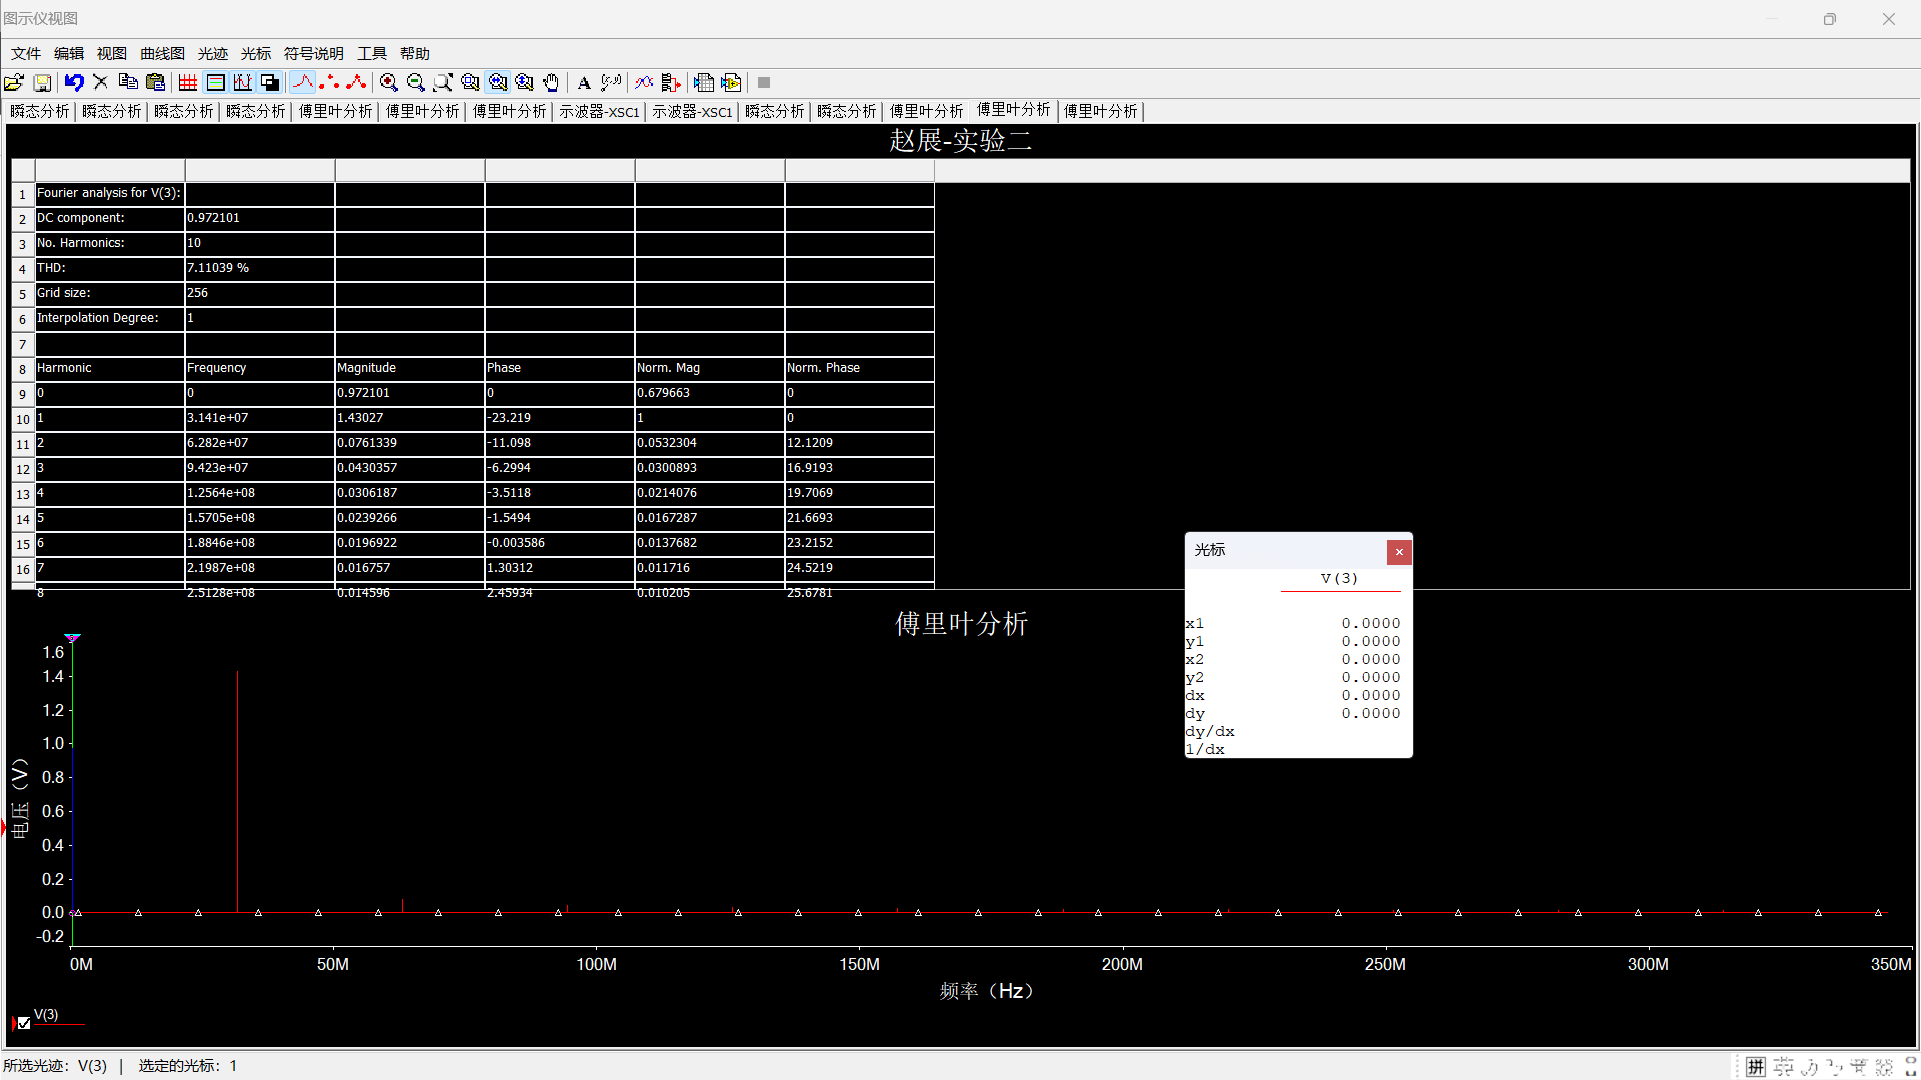
\includegraphics[width=0.6\textwidth]{16.png}
    \caption{傅里叶分析:欠压状态输入信号频谱}
    \label{img:16}
\end{figure}
\begin{figure}[htbp]
    \centering
    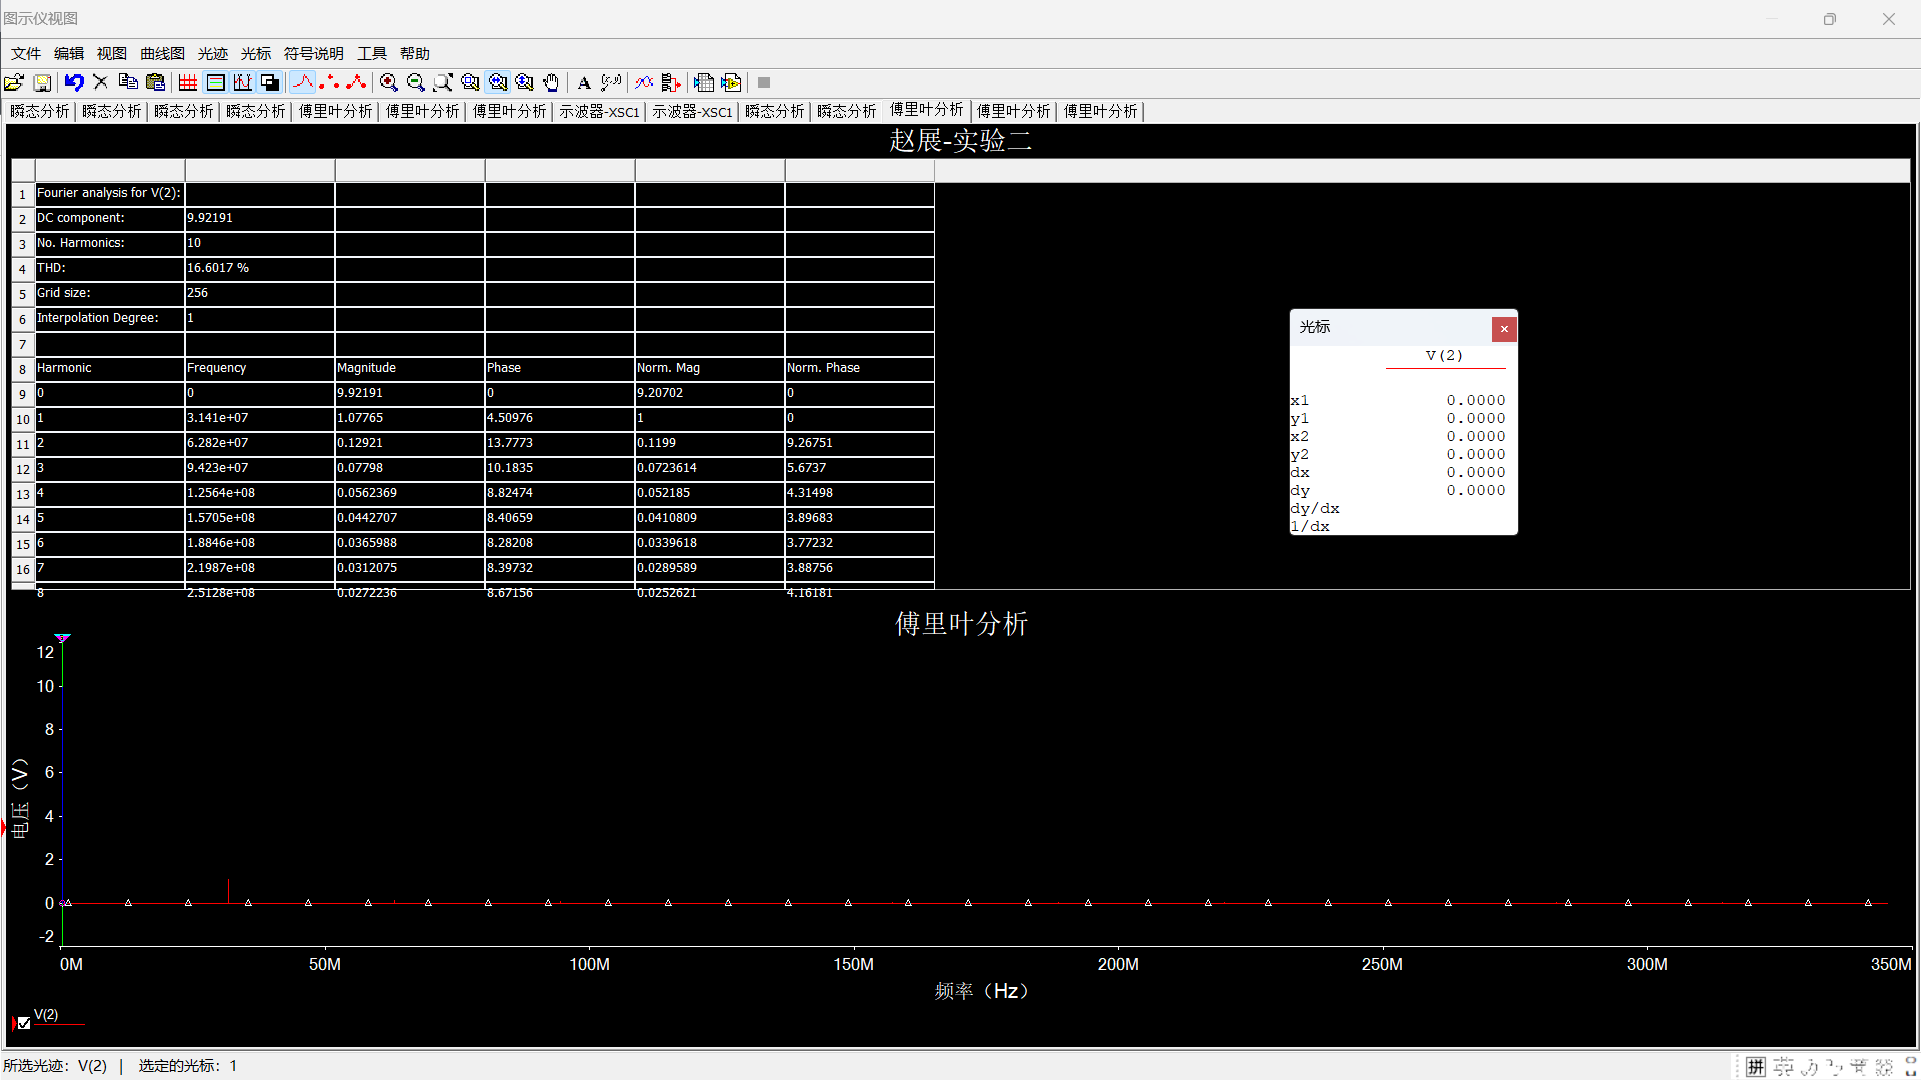
\includegraphics[width=0.6\textwidth]{17.png}
    \caption{傅里叶分析:欠压状态输出信号频谱}
    \label{img:17}
\end{figure}
启动傅里叶分析仿真,得到$i_c$、输入信号、输出信号的频谱如图\ref{img:15},\ref{img:16},\ref{img:17}所示,
可以看到,$i_c$频谱只剩下了一个频率分量,没有失真。
\begin{figure}[htbp]
    \centering
    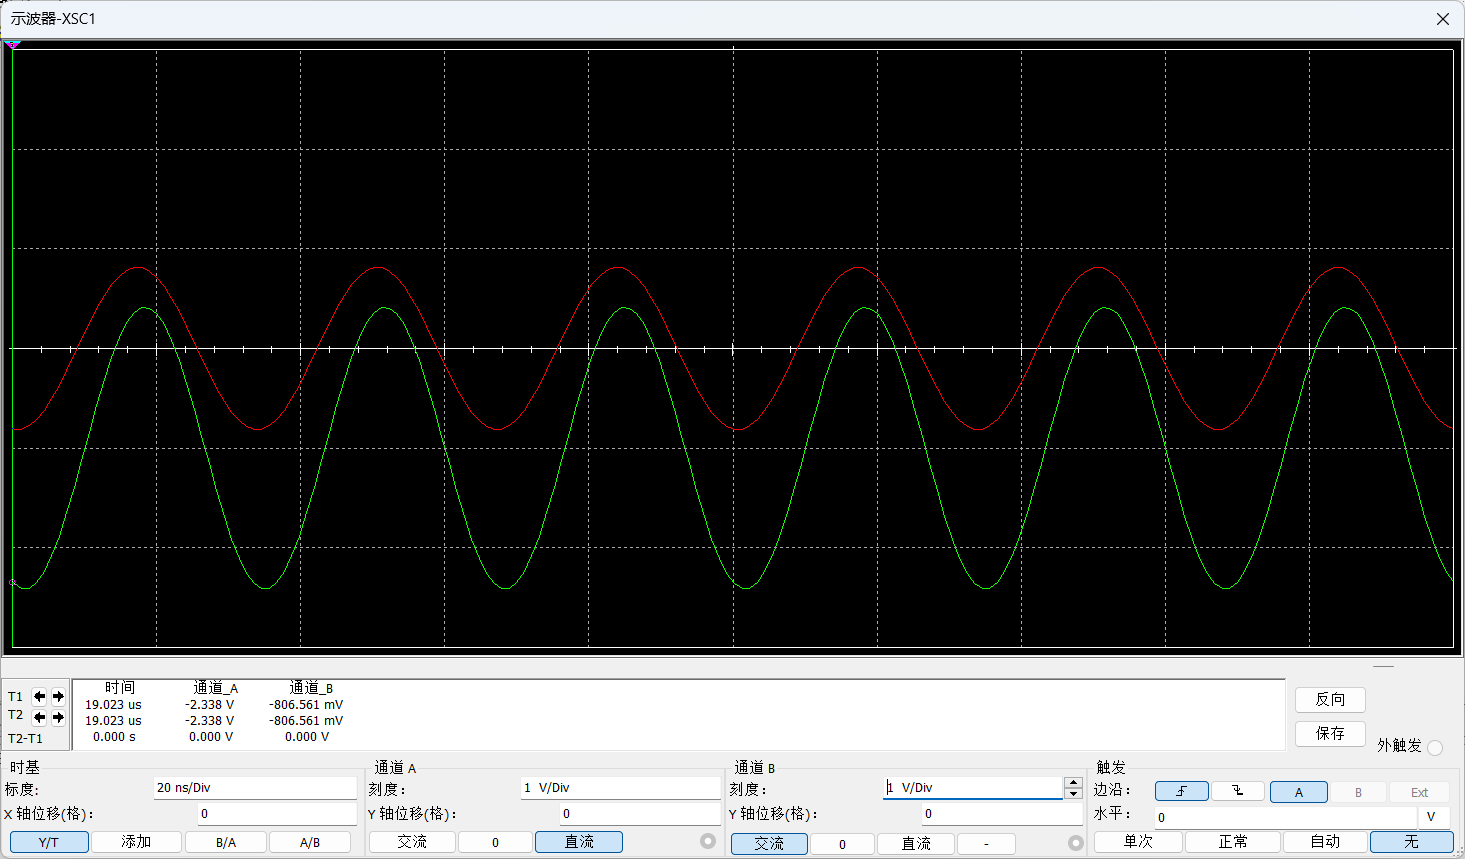
\includegraphics[width=0.8\textwidth]{18.png}
    \caption{示波器:欠压状态输入输出信号}
    \label{img:18}
\end{figure}
此时打开示波器查看输入输出信号的时域波形如图\ref{img:18}所示,可以看到信号无失真。
\newpage
\section{实验小结}
通过本次实验,我对Multisim的使用更加熟练,同时在高频谐振功率放大器这部分的知识也是又复习了一下,对其欠压、临界、过压的三个状态的了解更加深入了。
\end{document}